\documentclass{beamer}
\usetheme{Boadilla}

\usepackage[czech]{babel}
\usepackage{xcolor}
\usepackage{graphicx}
\usepackage{siunitx}

%pictures
\usepackage{tikz}
\usetikzlibrary{decorations.pathreplacing,angles,quotes,calc}
%checkboxes
\usepackage{pifont}
\usepackage{amssymb}

\title{Efekt úhlové rychlosti na odraz míčku}
\subtitle{První část experimentu a základ teorie}
\author{Jáchym Löwenhöffer}
\institute{GEVO JM}
\date{\today}

\begin{document}
  \begin{frame}
  \titlepage
 \end{frame}

 \begin{frame}{Outline}
  \tableofcontents
 \end{frame}

 \section{Uvedení do problému}
 
 \begin{frame}{Nastínění problému}
  \centering
  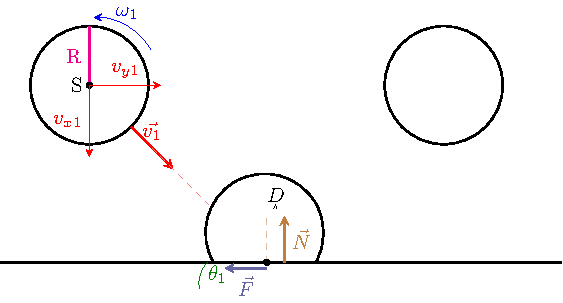
\includegraphics{diagram.pdf}\\
  \raggedright
  $\color{red}\vec{v_{1,2}}$ = rychlost před/po odrazu \\
  $\color{blue}\omega_{1,2}$ = spin před/po odrazu \\
  $\color[rgb]{0,0.5,0}\theta_{1,2}$ = úhel dopadu/odrazu \\
  
 \end{frame}

 \begin{frame}{Výzkumná otázka}
  \centering
  Jaký backspin je potřeba pro zpětný odraz míčku a jak ovlivňuje spin po
  odrazu? Pro všechny úhly odrazu
  ($\qty{0}{\degree}-\qty{90}{\degree}$) a vybrané
  rychlosti($\qty{1}{\meter\per\second} - \qty{10}{\meter\per\second}$).
 \end{frame}

 \section{Teorie} 

 \begin{frame}{Teorie}
  Triviální příklady:
  \begin{itemize}
   \item Když míček nepadá dolů nemá se od čeho odrazit 
   \item Bez úhlové rotace se úhel dopadu rovná úhlu odrazu
   \item Když míček letí rovnoběžně s povrchem nemůže se odrazit zpátky
   \item Když míček letí kolmo na povrch je velmi jednoduché aby se odrazil
    zpátky
  \end{itemize}
 \end{frame}

 \begin{frame}{Předpoklady}
 \begin{itemize}
  \item Deformuje se jen míček
  \item Popisujeme jen samotný odraz
  \item Normálová síla působí jen v jednom bodě
  \item Při odrazu dochází jen ke smýkání 
 \end{itemize}
\end{frame}

\section{Experimenty}

\begin{frame}{Simulace}
 \centering
\begin{tikzpicture}[
 block/.style={
      rectangle,
      draw=blue,
      thick,
      fill=blue!20,
      text width=5em,
      align=center,
      rounded corners,
      minimum height=2em
   },
   box/.style={
    rectangle,
    draw=black,
    text width = 5em,
    align = center,
    rounded corners,
    minimum height = 2em,
   }
 ]
 %počítač
 \node[block] (poc) at (0,0) {počítač};

 %input
 \node[box] (input) at
 ($(poc)+(-4,0)$){$\color{red}\vec{v_1}$, $\color{blue}\omega_1$, $\color[rgb]{0,0.5,0}\theta_1$};
 %output
 \node[box] (output) at ($(poc)+(4,0)$){$\color{red}\vec{v_2}$, $\color{blue}\omega_2$};

 %rovnice
 \node[box] (rovnice) at ($(poc)+(0,2)$){rovnice};
 %materiálové konstanty
 \node[box] (konst) at ($(poc)+(0,-2)$) [align=left] {materiálové \\ konstanty};

 %šipky
 \draw[thick,-stealth] (input) -- (poc);
 \draw[thick,-stealth] (poc) -- (output);

 \draw[thick,-stealth] (konst) -- (poc);
 \draw[thick,-stealth] (rovnice) -- (poc);
 \end{tikzpicture}

\end{frame}

 \begin{frame}{Výsledky}
 Pro materiálové konstanty relevantní pro golfový míček na žulovém povrchu:
 \[
  v_{x2} < 0 \Rightarrow \theta_1 > \qty{69}{\degree}
 \]
 Tedy směr odrazu není závislý ani na $v_{x1}$ ani na $\omega_1$.
\end{frame}

\section{Otázky}

\begin{frame}{Závěr}
 \textbf{Cíl:} pro některé míčky a povrchy být schopný předpovědět jakým směrem
 se míček odrazí a najít takový spin aby se vracel zpátky ($v_{x2}<0$).
 \vfill
 \textbf{Postup:}\\
 \begin{itemize}
  \item[\rlap{\raisebox{0.3ex}{\hspace{0.4ex}\tiny \ding{52}}}$\square$]
  Simulace pro jednoduché podmínky
  
  \item[\rlap{\raisebox{0.3ex}{\hspace{0.4ex}\tiny \ding{52}}}$\square$]
  Základy teorie 
 \item[$\square$] Rozšířit simulaci na větší množství případů
 \item[$\square$] Rozlišit jaký bude průběh odrazu
 \item[$\square$] Porovnat simulovaná data s reálnými (ne nutně mými)
 \end{itemize}

\end{frame}
\end{document}

